\documentclass{beamer}
\usepackage[utf8]{inputenc}

\usetheme{Madrid}
\usecolortheme{default}
\usepackage{amsmath,amssymb,amsfonts,amsthm}
\usepackage{txfonts}
\usepackage{tkz-euclide}
\usepackage{listings}
\usepackage{adjustbox}
\usepackage{array}
\usepackage{tabularx}
\usepackage{gvv}
\usepackage{lmodern}
\usepackage{circuitikz}
\usepackage{tikz}
\usepackage{graphicx}

\setbeamertemplate{page number in head/foot}[totalframenumber]

\usepackage{tcolorbox}
\tcbuselibrary{minted,breakable,xparse,skins}



\definecolor{bg}{gray}{0.95}
\DeclareTCBListing{mintedbox}{O{}m!O{}}{%
  breakable=true,
  listing engine=minted,
  listing only,
  minted language=#2,
  minted style=default,
  minted options={%
    linenos,
    gobble=0,
    breaklines=true,
    breakafter=,,
    fontsize=\small,
    numbersep=8pt,
    #1},
  boxsep=0pt,
  left skip=0pt,
  right skip=0pt,
  left=25pt,
  right=0pt,
  top=3pt,
  bottom=3pt,
  arc=5pt,
  leftrule=0pt,
  rightrule=0pt,
  bottomrule=2pt,

  colback=bg,
  colframe=orange!70,
  enhanced,
  overlay={%
    \begin{tcbclipinterior}
    \fill[orange!20!white] (frame.south west) rectangle ([xshift=20pt]frame.north west);
    \end{tcbclipinterior}},
  #3,
}
\lstset{
    language=C,
    basicstyle=\ttfamily\small,
    keywordstyle=\color{blue},
    stringstyle=\color{orange},
    commentstyle=\color{green!60!black},
    numbers=left,
    numberstyle=\tiny\color{gray},
    breaklines=true,
    showstringspaces=false,
}
%------------------------------------------------------------
%This block of code defines the information to appear in the
%Title page
\title %optional
{1.9.1}
\date{August  2025}
%\subtitle{A short story}

\author % (optional)
{BEERAM MADHURI - EE25BTECH11012}



\begin{document}


\frame{\titlepage}
\begin{frame}{Question}
The distance between the points $(m, -n)$ and $(-m, n)$ is \underline{\hspace{2cm}}
 
\end{frame}
 
\begin{frame}{given data}
 
\text let \textbf{A} and \textbf{B} be the vectors such that:
\begin{table}[h!]
    \centering
    \begin{tabular}{|c|c|}
\hline
\textbf{Name} & \textbf{Value} \\ \hline
$\vec{A}$ & $\myvec{2 & 1 \\0 & 3}$ \\ \hline
\end{tabular}

    \caption{Variables used}
    \label{table 1.9.1}
\end{table}


   
\end{frame}

\begin{frame}{Formula} 
Norm of \textbf{A} - \textbf{B} is given by:
\begin{align*}
\| \textbf{A} - \textbf{B} \| &= \sqrt{\|\textbf{A}\|^2 + \|\textbf{B}\|^2 - 2 A^\top\textbf{B} }\\
 \end{align*}
 \end{frame}
 

\begin{frame}{solution}
    \frametitle{finding distance between \textbf{A} and \textbf{B}}
\begin{align*}
\| \textbf{A} - \textbf{B} \| &= \sqrt{\|\textbf{A}\|^2 + \|\textbf{B}\|^2 - 2 A^\top\textbf{B} }\\
&= \sqrt{(m^2 + n^2) - 2(-m^2 - n^2) + m^2 + n^2} \\
&= \sqrt{4(m^2+n^2)} \\
&= 2\sqrt{m^2+n^2}
\end{align*}

\text Hence Distance between \textbf{A} and \textbf{B} is $2\sqrt{m^2+n^2}$.
\end{frame}


\begin{frame}[fragile]
    \frametitle{Python Code}
    \begin{lstlisting}
 import matplotlib.pyplot as plt
import numpy as np

# Define m and n
m = 3
n = 4

# Define the points A and B
A = np.array([m, -n])
B = np.array([-m, n])

\end{lstlisting}
\end{frame}

\begin{frame}[fragile]
    \frametitle{Python Code}

    \begin{lstlisting}
# Calculate the distance between A and B
distance = 2 * np.sqrt(m**2 + n**2)
print(f"Distance between A{tuple(A)} and B{tuple(B)} is: {distance}")

# Create the plot
fig, ax = plt.subplots(figsize=(8, 6))

    \end{lstlisting}
\end{frame}

\begin{frame}[fragile]
    \frametitle{Python Code}

    \begin{lstlisting}
# Plot points A and B
ax.scatter(A[0], A[1], color='red', s=100, label=f'A = {tuple(A)}')
ax.scatter(B[0], B[1], color='blue', s=100, label=f'B = {tuple(B)}')

# Draw line segment between A and B
ax.plot([A[0], B[0]], [A[1], B[1]], 'k--', alpha=0.6, label='Line Segment AB')

# Plot origin for reference
ax.scatter(0, 0, color='black', s=80, label='Origin (0,0)')
    \end{lstlisting}
\end{frame}

\begin{frame}[fragile]
    \frametitle{Python Code}

    \begin{lstlisting}
# Add labels for points
ax.text(A[0] + 0.2, A[1], 'A', fontsize=14)
ax.text(B[0] + 0.2, B[1], 'B', fontsize=14)
ax.text(0.2, 0.2, 'O', fontsize=14)
\end{lstlisting}
\end{frame}

 
\begin{frame}[fragile]
    \frametitle{Python Code}

    \begin{lstlisting}
# Set plot limits with some margin
margin = max(abs(m), abs(n)) + 1
ax.set_xlim(-margin, margin)
ax.set_ylim(-margin, margin)
\end{lstlisting}
\end{frame}
\begin{frame}[fragile]
    \frametitle{Python Code}

    \begin{lstlisting}
# Add grid, title, labels, legend
ax.grid(True, linestyle='--', alpha=0.5)
ax.set_title('Distance Between Points A and B', fontsize=16)
ax.set_xlabel('X-axis', fontsize=12)
ax.set_ylabel('Y-axis', fontsize=12)
ax.legend()

# Equal aspect ratio
ax.set_aspect('equal', adjustable='box')

plt.show()
\end{lstlisting}
\end{frame}

\begin{frame}[fragile]
\frametitle{C Code}
\begin{lstlisting}
  
#include <stdio.h>
#include <math.h>
int main() {
    double m, n, distance;
    // Input values for m and n
    printf("Enter the value of m: ");
    scanf("%lf", &m);
\end{lstlisting}
\end{frame}

\begin{frame}[fragile]
\frametitle{C Code}
\begin{lstlisting}
    printf("Enter the value of n: ");
    scanf("%lf", &n);
    // Calculate distance using the formula
    distance = 2 * sqrt(m * m + n * n);
    // Print the result
    printf("Distance between the points (%.2lf, %.2lf) and (%.2lf, %.2lf) is: %.4lf\n",
           m, -n, -m, n, distance);
    return 0;
}


\end{lstlisting}

\end{frame}


\begin{frame}[fragile]
\frametitle{Python and C Code}

\begin{lstlisting}
import ctypes
import platform

# --- 1. Load the shared library ---
if platform.system() == "Windows":
    lib_path = "./libdistance.dll"
else:
    lib_path = "./libdistance.so"

try:
    lib = ctypes.CDLL(lib_path)
except OSError as e:
    print(f"Error loading library: {e}")
    print("Have you compiled distance_calc.c?")
    exit()
\end{lstlisting}
\end{frame}

\begin{frame}[fragile]
\frametitle{Python and C Code}

\begin{lstlisting}
# --- 2. Define the function signature ---
# Set the argument types
lib.calculate_distance.argtypes = [ctypes.c_double, ctypes.c_double]

# IMPORTANT: Set the return type.
# This tells ctypes that the C function returns a double value.
lib.calculate_distance.restype = ctypes.c_double
\end{lstlisting}
\end{frame}

\begin{frame}[fragile]
\frametitle{Python and C Code}

\begin{lstlisting}
# --- 3. Get input from the user in Python ---
try:
    m_val = float(input("Enter the value of m: "))
    n_val = float(input("Enter the value of n: "))
except ValueError:
    print("Invalid input. Please enter numbers.")
    exit()
\end{lstlisting}
\end{frame}

\begin{frame}[fragile]
\frametitle{Python and C Code}

\begin{lstlisting}
# --- 4. Call the C function and get the returned value ---
distance = lib.calculate_distance(m_val, n_val)

# --- 5. Print the result ---
print("\n--- Calculation performed by C ---")
print(f"Distance between the points ({m_val:.2f}, {-n_val:.2f}) and ({-m_val:.2f}, {n_val:.2f}) is: {distance:.4f}")
\end{lstlisting}

\end{frame}

\begin{figure}[H]
    \centering
    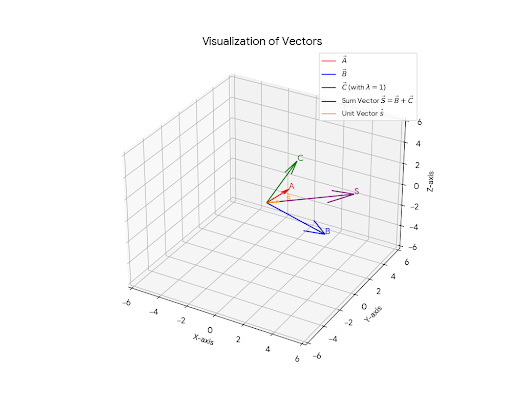
\includegraphics[width=0.7\columnwidth]{Fig.png}
    \caption{Plot}
    \label{fig:placeholder}
\end{figure}


\end{document}